\section{Task 1: TLS Client}
\subsection{Task 1.a: TLS handshake}
%
I used the command below to communicate with {\fontfamily{qcr}\selectfont tuni.fi}
server.

\begin{lstlisting}[language=bash]
    python3 handshake.py tuni.fi
\end{lstlisting}

\begin{lstlisting}[caption=TLS Hanshake negotiation aand certificate log,
    label={lst:handshake_log}]
Cipher used: ('ECDHE-RSA-AES128-GCM-SHA256', 'TLSv1.2', 128)
=== Server hostname: tuni.fi
=== Server certificate:
{'OCSP': ('http://GEANT.ocsp.sectigo.com',),
 'caIssuers': ('http://GEANT.crt.sectigo.com/GEANTOVRSACA4.crt',),
 'crlDistributionPoints': ('http://GEANT.crl.sectigo.com/GEANTOVRSACA4.crl',),
 'issuer': ((('countryName', 'NL'),),
            (('organizationName', 'GEANT Vereniging'),),
            (('commonName', 'GEANT OV RSA CA 4'),)),
 'notAfter': 'Jun 21 23:59:59 2023 GMT',
 'notBefore': 'Jun 21 00:00:00 2022 GMT',
 'serialNumber': '169B2623CE1AFC3A7FDDDFD89EB7437E',
 'subject': ((('countryName', 'FI'),),
             (('stateOrProvinceName', 'Pirkanmaa'),),
             (('organizationName', 'Tampere University Foundation sr'),),
             (('commonName', 'www.tuni.fi'),)),
 'subjectAltName': (('DNS', 'www.tuni.fi'), ('DNS', 'tuni.fi')),
 'version': 3}
[{'issuer': ((('countryName', 'US'),),
             (('stateOrProvinceName', 'New Jersey'),),
             (('localityName', 'Jersey City'),),
             (('organizationName', 'The USERTRUST Network'),),
             (('commonName', 'USERTrust RSA Certification Authority'),)),
  'notAfter': 'Jan 18 23:59:59 2038 GMT',
  'notBefore': 'Feb  1 00:00:00 2010 GMT',
  'serialNumber': '01FD6D30FCA3CA51A81BBC640E35032D',
  'subject': ((('countryName', 'US'),),
  (('stateOrProvinceName', 'New Jersey'),),
  (('localityName', 'Jersey City'),),
  (('organizationName', 'The USERTRUST Network'),),
  (('commonName', 'USERTrust RSA Certification Authority'),)),
    'notAfter': 'Jan 18 23:59:59 2038 GMT',
    'notBefore': 'Feb  1 00:00:00 2010 GMT',
    'serialNumber': '01FD6D30FCA3CA51A81BBC640E35032D',
    'subject': ((('countryName', 'US'),),
    (('stateOrProvinceName', 'New Jersey'),),
    (('localityName', 'Jersey City'),),
    (('organizationName', 'The USERTRUST Network'),),
    (('commonName', 'USERTrust RSA Certification Authority'),)),
    'version': 3}]
\end{lstlisting}

The agreed ciphersuite and the server certificate are shown in
\autoref{lst:handshake_log}. The agreed ciphersuite is ``ECDHE-RSA-AES128-GCM-SHA256'',
which means that:

\begin{itemize}
    \item Key Exchange: Elliptic Curve Diffie-Hellman Ephemeral (ECDHE).
    \item Authentication (Public-Key Digital Signature): Rivest Shamir Adleman algorithm (RSA).
    \item Encryption: Advanced Encryption Standard with 128bit key in Galois Counter mode
    (AES128-GCM).
    \item Hash: Secure Hash Algorithm 256 (SHA256)
\end{itemize}


{\fontfamily{qcr}\selectfont /etc/ssl/certs}
is the directory storing CA certificates used to validate other peers' certificates.

%%% List of figures showing TCP and TLS packets
\begin{figure}
    \centering
    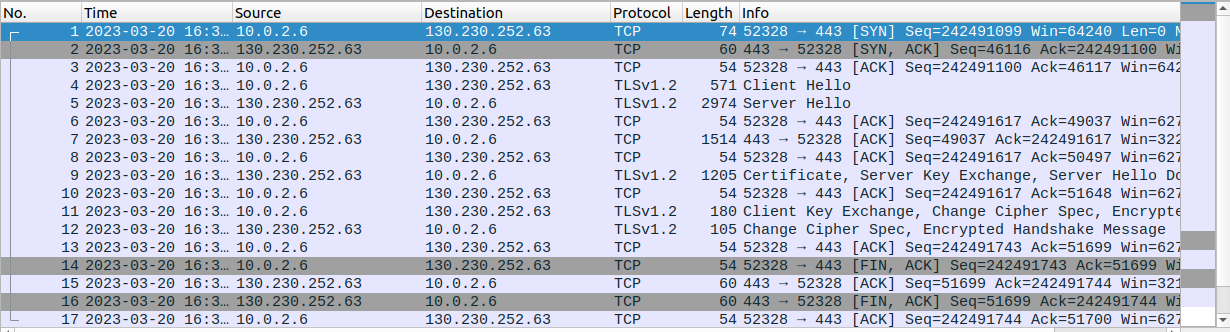
\includegraphics[height=\textheight,width=\textwidth,keepaspectratio]
    {figures/wireshark_packets.png}
    \caption{All TCP and TLS packets were transmitted while
    {\fontfamily{qcr}\selectfont handshake.py} was running.}
    \label{fig:all_packets}
\end{figure}


%%% End of figures listing

Some clarification:
\begin{itemize}
    \item Host machine IP address: 10.0.2.6
    \item {\fontfamily{qcr}\selectfont tuni.fi} server IP address: 130.230.252.63
\end{itemize}

As TLS is built on top of the Transmission Control Protocol (TCP), there had been a TCP 3-way
handshake before a TLS was initialized (see \autoref{fig:all_packets}).Firstly, the client
sent a segment with SYN to the web server and with a \emph{Seq} number (242491099)
for initializing a communication. Then, the server responded with a SYN-ACK with a pair of
\emph{Seq} and \emph{Ack} number. In the response, \emph{Ack} is the one-incremented number
of the previous \emph{Seq} number (242491100) in the initializing request, and the new \emph{Seq} number
here (46116) was generated by the server. Finally, after receiving the SYN-ACK signal, the client
sent back the ACK with the \emph{Seq} number which equals to the previous \emph{Ack} number (242491100)
and the \emph{Ack} number which is a one-incremented of the previous \emph{Seq} number (46117).
So the TCP 3-way handshake protocol ended here.

\begin{figure}
    \centering
    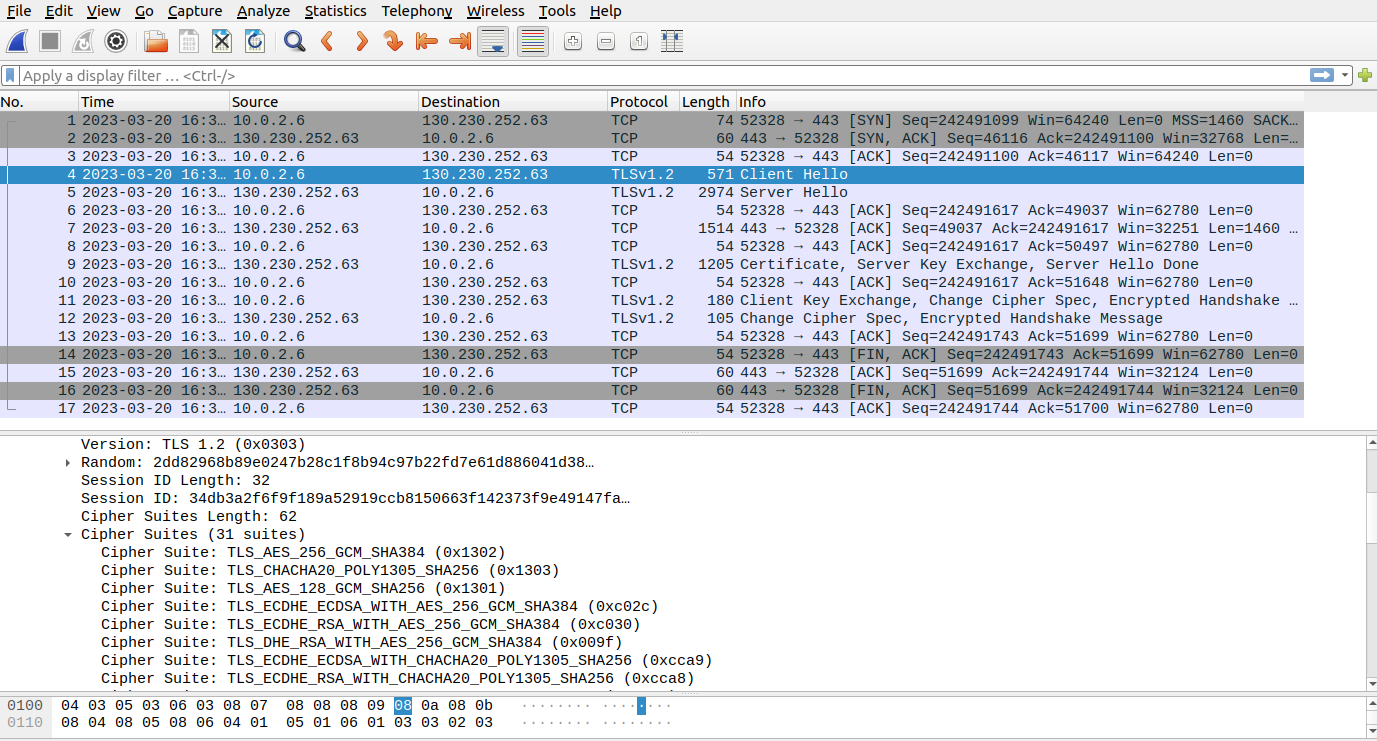
\includegraphics[height=\textheight,width=\textwidth,keepaspectratio]
    {figures/client_hello.png}
    \caption{`Client Hello' message of a TLS handshake.}
    \label{fig:client_hello_handshake}
\end{figure}

\begin{figure}
    \centering
    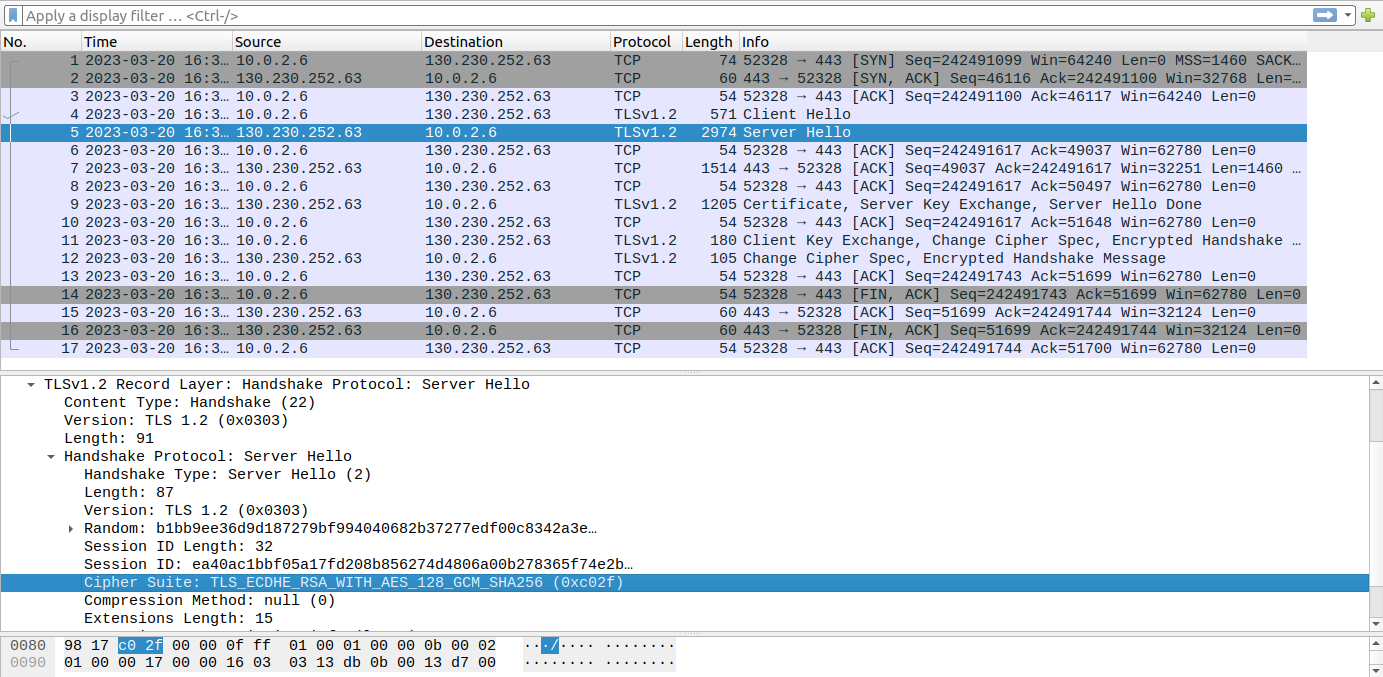
\includegraphics[height=\textheight,width=\textwidth,keepaspectratio]
    {figures/server_hello.png}
    \caption{`Server Hello' message of a TLS handshake.}
    \label{fig:server_hello_handshake}
\end{figure}

\begin{figure}
    \centering
    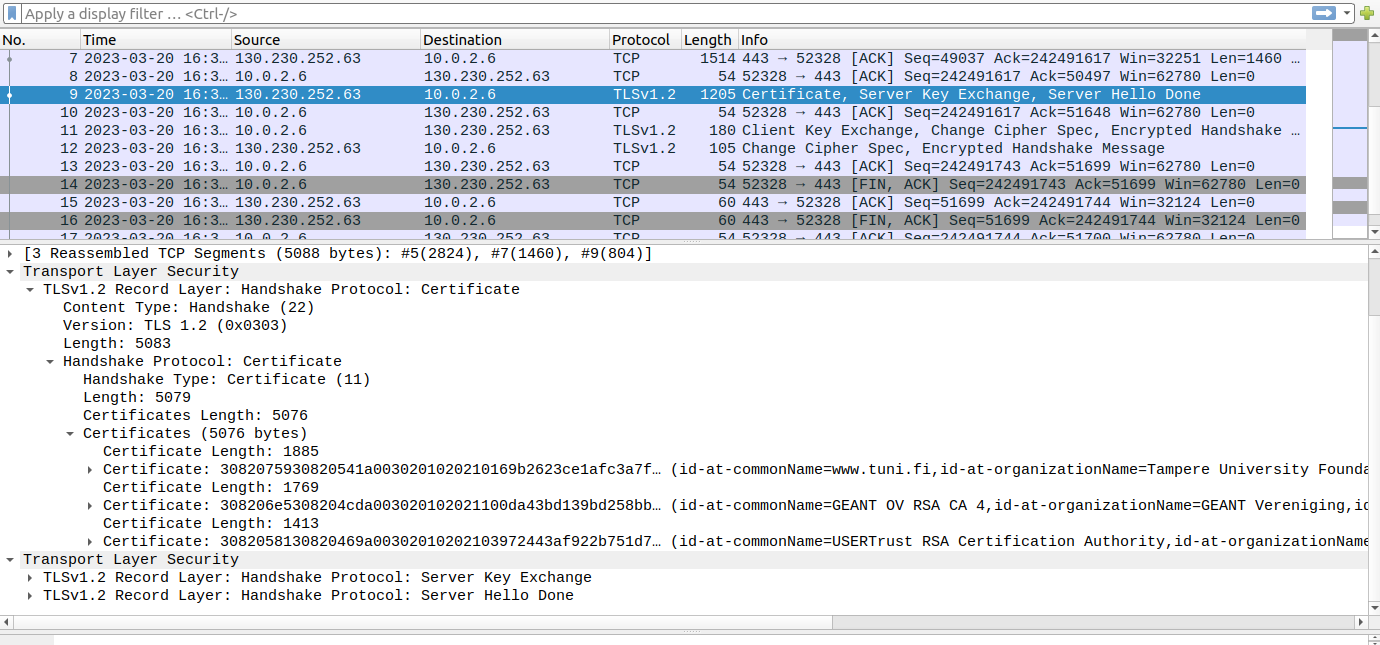
\includegraphics[height=\textheight,width=\textwidth,keepaspectratio]
    {figures/certificate_tls.png}
    \caption{`Certificate' segment of a TLS handshake.}
    \label{fig:cert_tls}
\end{figure}

Next, the TLS 1.2 handshake protocol started. Firstly, The client sent `Client Hello' message to
initiate the handshake. In this message, the client include its supported TLS version, supported
cipher suites (31 suites in this case), and a random number (see \autoref{fig:client_hello_handshake}). Next, the server
responded with a `Server Hello' message which contains the selected cipher suite and a
random number generated by the server (see \autoref{fig:server_hello_handshake}). Along with
that, the server also sent `Certificate', `Server Key Exchange', and `Server Hello Done'
messages. In the `Certificate' segment, information of SSL certifcates for verification were inlcuded
. As shown in \autoref{fig:cert_tls}, there are up to 3 certificates for verifying each other.
The reason is that a certificate of a web server is signed by an issuer A, and the certificate
of the issuer A is signed by a issuer B, and so forth until a certificate of the root CA is verified.
In each certificate, public-key elements (modulus, publicExponent, algorithm, etc.), subject, issuer,
etc. are included. In the `Server Key Exchange', parameters for Elliptic Curve Diffie-Hellman
Key Exchange (ECDKE) for exchanging the \emph{PreMasterSecret}, and the digital signature of
the message (see \autoref{fig:server_key_exchange_tls}).


\begin{figure}
    \centering
    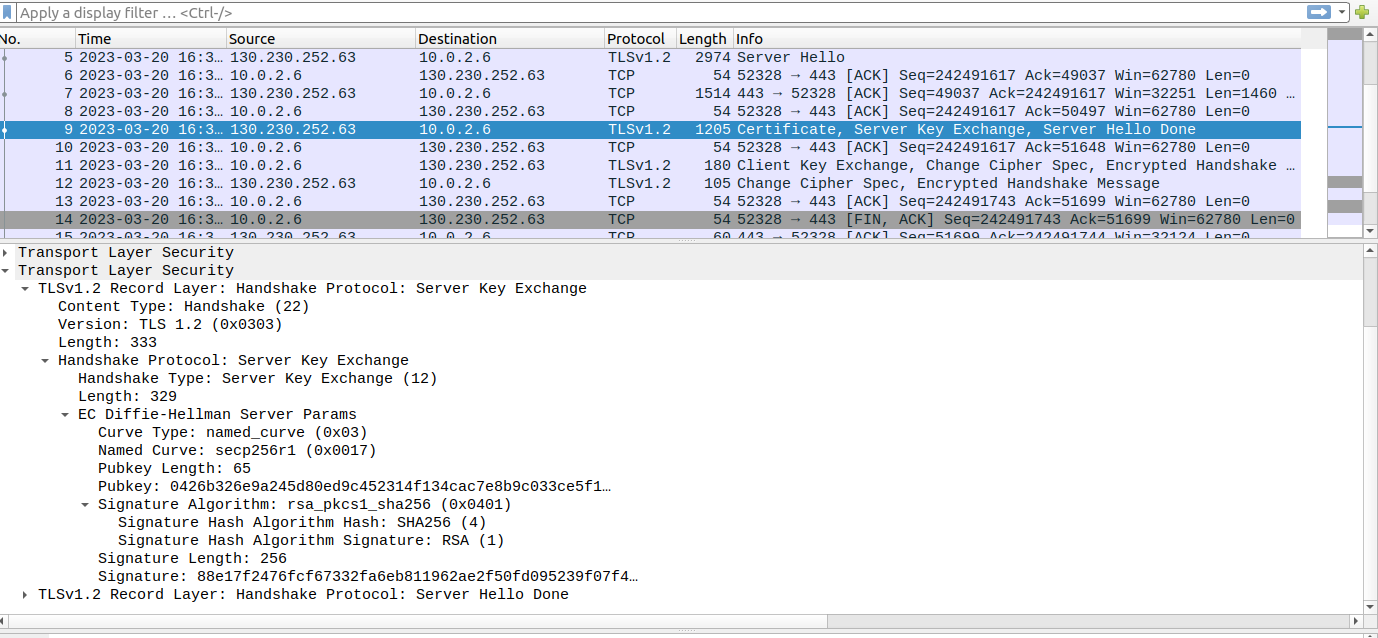
\includegraphics[height=\textheight,width=\textwidth,keepaspectratio]
    {figures/server_key_exchange.png}
    \caption{`Server Key Exchange' segment of a TLS handshake.}
    \label{fig:server_key_exchange_tls}
\end{figure}

\begin{figure}
    \centering
    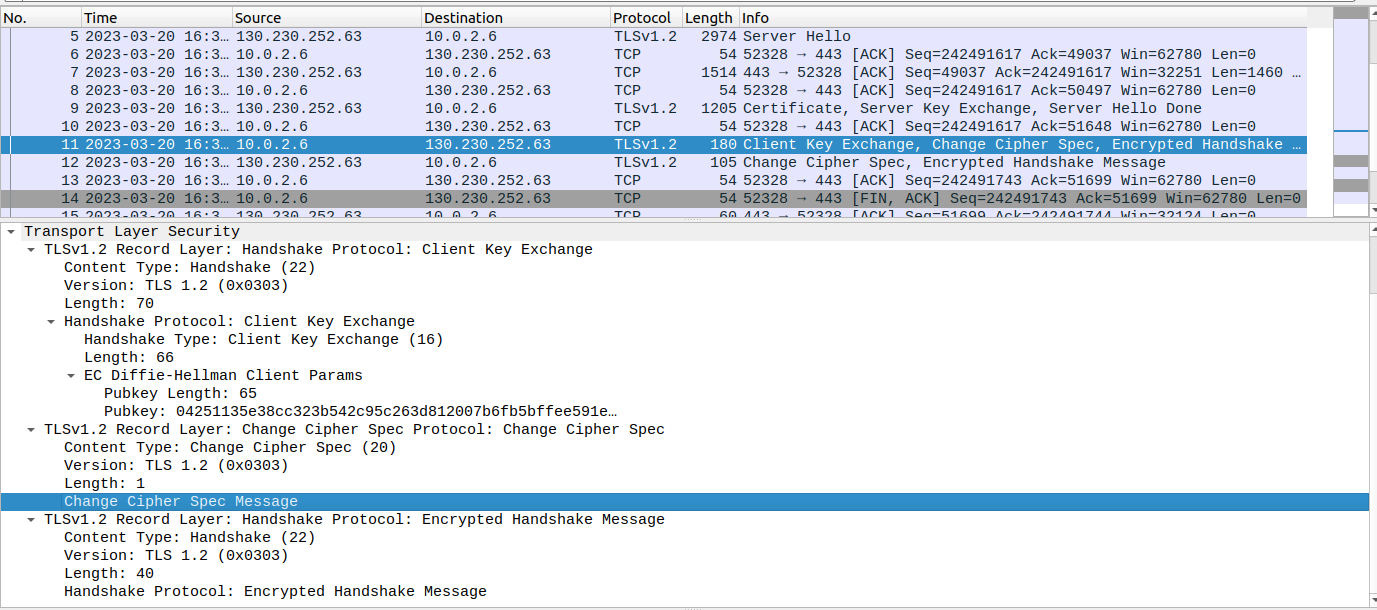
\includegraphics[height=\textheight,width=\textwidth,keepaspectratio]
    {figures/client_key_exchange.png}
    \caption{`Client Key Exchange', `Change Cipher Spec', and `Encrypted Handshake Message'
    segments of a TLS handshake from the client's side.}
    \label{fig:client_key_exchange_more_tls}
\end{figure}

\begin{figure}
    \centering
    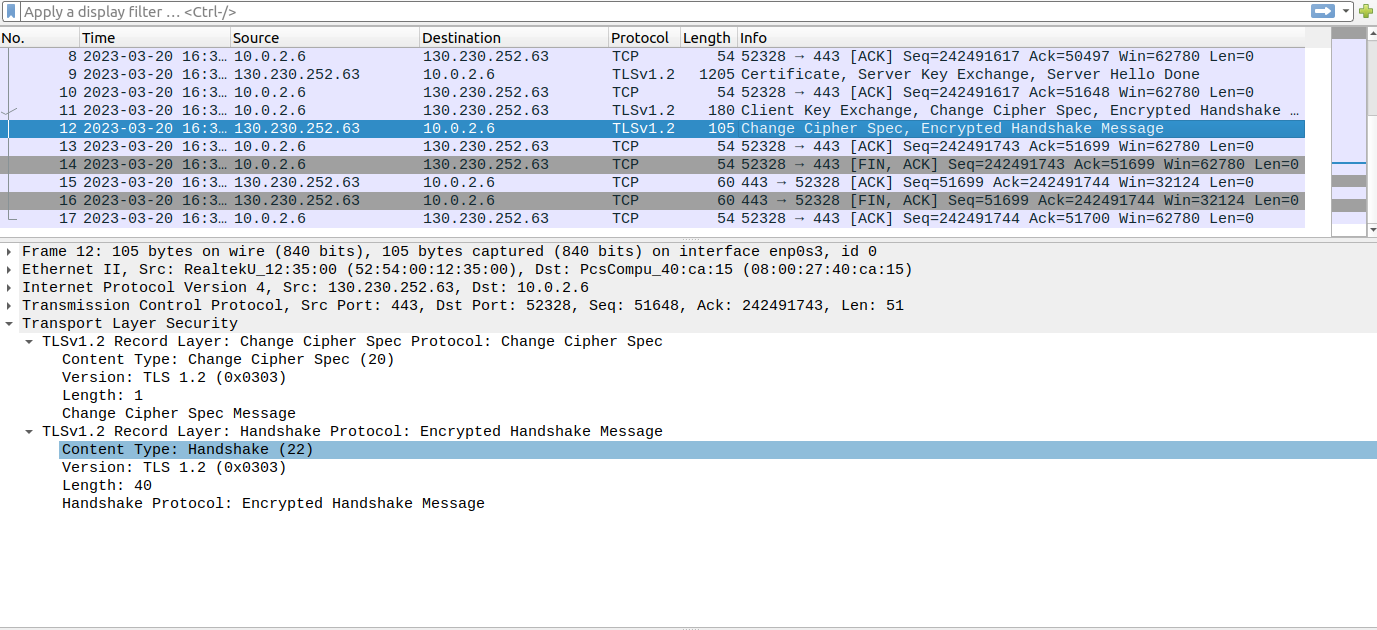
\includegraphics[height=\textheight,width=\textwidth,keepaspectratio]
    {figures/server_change_cipher_spec_more.png}
    \caption{`Change Cipher Spec' and `Encrypted Handshake Message' segments of a
    TLS handshake from the server's side.}
    \label{fig:server_change_cipher_spec_more_tls}
\end{figure}

Next, a `Server Hello Done' was sent to inform that the server had sent anything needed
for the next step. Then from the client's side, `Client Key Exchange', `Change Cipher Spec',
and `Encrypted Handshake Message' were replied (see \autoref{fig:client_key_exchange_more_tls}).
`Client Key Exchange' is replied, at this point,
the client and the server both have the same \emph{PreMasterSecret} which was combined with
random numbers generated in `Client Hello' and `Server Hello' to produce the \emph{MasterSecret},
a symmetric key used for later data encryption/decrytion. `Change Cipher Spec' from the client
informs that the client now had all information needed for starting encryption data. And
`Encrypted Handshake Message' is the encrypted message, with key is the \emph{MasterSecret},
that summerizes all of the messages in the handshake so far. Then, the server responded with
the same segments, `Change Cipher Spec' and `Encrypted Handshake Message'
(see \autoref{fig:server_change_cipher_spec_more_tls}). So at this point,
the TLS 1.2 handshake protocol was finished, data packets between the server and the client
later will be encrypted with the pre-agreed parameters and cryptographic algorithms.